\chapter{تصنيف العالم الحي}\label{ch:b1:classifying-biodiversity}

سُمّي نحو \num{2} مليون \omterm{def:b1:classifying-biodiversity:species}{نوع}، ويُضاف كل سنة نحو
\num{18000}؛ ويُقدَّر عدد \omterm{def:b1:classifying-biodiversity:species}{الأنواع} الموجودة بنحو
\num{9} ملايين \omterm{def:b1:cell-unit-of-life:prokeuk}{لحقيقيات النواة} وحدها، ولا أحد يعرف كم من
البكتيريا. والاسم بداية فحسب: فالبيولوجي يريد أن يعرف
أي \omterm{def:b1:classifying-biodiversity:species}{الأنواع} أقرب إلى أي، والجواب شجرة، لأن
\omterm{def:b1:classifying-biodiversity:species}{الأنواع} تربطها الأصول المشتركة. ويعطي هذا الفصل قواعد
التسمية، والطرائق التي تُستنبط بها القرابات من
الصفات --- والمعيار، وهو \omterm{def:b1:classifying-biodiversity:parsimony}{الاقتصاد}، الذي تُحكَّم به الشجرات
المتنافسة --- وشكل شجرة الحياة كما تُفهم اليوم،
وحال جرد ما يعيش.

\section{الأنواع والأسماء}

\begin{definition}[النوع]\label{def:b1:classifying-biodiversity:species}
\index{نوع}\index{مفهوم النوع البيولوجي}
\emph{النوع}، وفق \emph{مفهوم النوع البيولوجي}، مجموعة من
\omterm{def:b1:populations:population}{الجمهرات} يستطيع أفرادها التزاوج فيما بينهم وإنتاج نسل خصب
وهم معزولون تكاثريًا عن سائر المجموعات المماثلة.
ولا يمكن تطبيق المفهوم على \omterm{def:b1:organism-environment:organism}{الكائنات} التي لا تتكاثر
جنسيًا (أكثر البكتيريا، وكثير من الطلائعيات وبعض النباتات والحيوانات)،
ولا على الأحافير، ولا على \omterm{def:b1:populations:population}{الجمهرات} التي لا تلتقي أبدًا؛ فهناك يُعرَّف النوع
بشكله الظاهري (المفهوم \emph{الشكلي})، أو بسلالته المتميزة على شجرة (المفهوم
\emph{النشوئي})، أو بعتبة من التباعد الوراثي. وكل المفاهيم تحاول تسمية
الشيء نفسه: سلالة تتطور مستقلة عن غيرها.
\end{definition}

\begin{definition}[التسمية والمراتب]\label{def:b1:classifying-biodiversity:nomenclature}
\index{تسمية ثنائية}\index{وحدة تصنيفية}\index{جنس}\index{عينة نمطية}
لكل \omterm{def:b1:classifying-biodiversity:species}{نوع} اسم \emph{ثنائي}: اسم
\emph{جنسه} (بحرف كبير) يليه نعت نوعي، وكلاهما
مائل --- \emph{Homo sapiens}، و\emph{Quercus robur}،
و\emph{Escherichia coli} --- ويليهما غالبًا مؤلف الوصف وسنته.
والنظام، الذي ثبّته لينيوس سنة 1753 (للنباتات) و
1758 (للحيوانات)، يعشّش \omterm{def:b1:classifying-biodiversity:species}{الأنواع} في تدرج من \emph{المراتب}: الجنس،
والفصيلة، والرتبة، والطائفة، والشعبة (أو القسم)، والمملكة، والمجال. والمجموعة
عند أي مرتبة \emph{وحدة تصنيفية}. وكل اسم مرتبط بعينة \emph{نمطية}، مودعة في متحف أو معشبة، تثبّت ما يشير إليه
الاسم؛ وأقدم اسم صالح له الأولوية؛ والقواعد
مقننة حتى يكون للكائن الواحد اسم واحد في العالم كله. والمراتب
أعراف --- فليست ثمة خاصة تشترك فيها كل الفصائل ولا يملكها
جنس؛ \omterm{def:b1:classifying-biodiversity:species}{والنوع} وحده وحدة طبيعية.
\end{definition}

\begin{omfigure}
\begin{tikzpicture}[font=\footnotesize, line cap=round]
  \draw[thick, omDef!60!black, fill=omDef!6, rounded corners=4pt] (0,0) rectangle (11.4,5.4); \node[anchor=north west, omDef!80!black] at (0.1,5.35) {مجال Eukarya};
  \draw[thick, omDef!60!black, fill=omDef!10, rounded corners=4pt] (0.4,0.3) rectangle (11.0,4.75); \node[anchor=north west, omDef!80!black] at (0.5,4.7) {مملكة Animalia};
  \draw[thick, omProp!70!black, fill=omProp!10, rounded corners=4pt] (0.8,0.6) rectangle (10.6,4.1); \node[anchor=north west, omProp!80!black] at (0.9,4.05) {شعبة Chordata};
  \draw[thick, omProp!70!black, fill=omProp!18, rounded corners=4pt] (1.2,0.9) rectangle (10.2,3.45); \node[anchor=north west, omProp!80!black] at (1.3,3.4) {طائفة Mammalia};
  \draw[thick, omThm!70!black, fill=omThm!10, rounded corners=4pt] (1.6,1.2) rectangle (9.8,2.8); \node[anchor=north west, omThm!80!black] at (1.7,2.75) {رتبة Carnivora};
  \draw[thick, omThm!70!black, fill=omThm!20, rounded corners=4pt] (2.0,1.4) rectangle (5.6,2.3); \node[anchor=north west, omThm!80!black] at (2.1,2.25) {فصيلة Felidae};
  \node[anchor=west] at (2.1,1.65) {جنس \emph{Felis}: \emph{F.~catus}};
  \draw[thick, omThm!70!black, fill=omThm!20, rounded corners=4pt] (5.9,1.4) rectangle (9.5,2.3); \node[anchor=north west, omThm!80!black] at (6.0,2.25) {فصيلة Canidae};
  \node[anchor=west] at (6.0,1.65) {جنس \emph{Canis}: \emph{C.~lupus}};
\end{tikzpicture}

{\small المراتب المعشَّشة في تدرج لينيوس، للقط
والذئب. وكل صندوق \omterm{def:b1:classifying-biodiversity:nomenclature}{وحدة تصنيفية}؛ والاسم الثنائي يسمّي \omterm{def:b1:classifying-biodiversity:nomenclature}{الجنس}
\omterm{def:b1:classifying-biodiversity:species}{والنوع}.}
\end{omfigure}

\begin{omfigure}
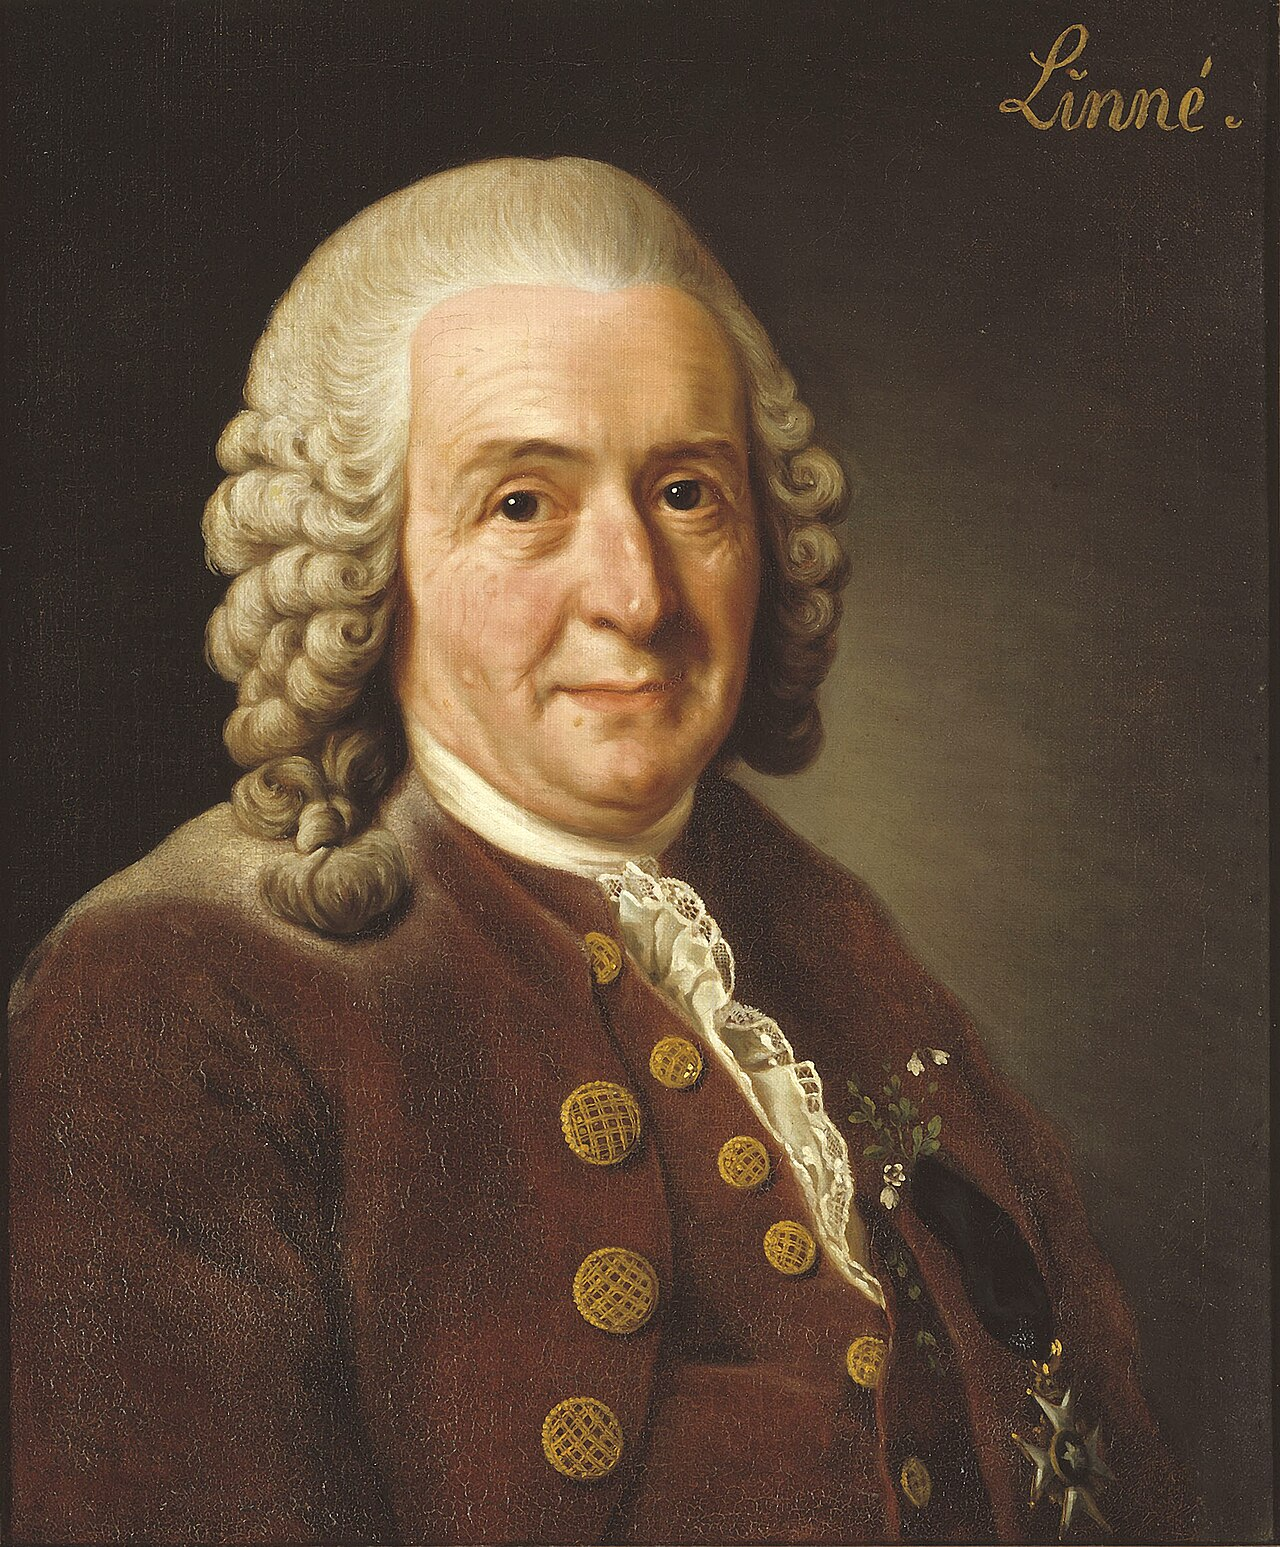
\includegraphics[width=0.36\linewidth]{images/book3/linnaeus.jpg}

{\small كارل لينيوس (Carl Linnaeus) (1707--1778)، وكتابه \emph{Species Plantarum}
سنة 1753 والطبعة العاشرة من \emph{Systema Naturae} سنة 1758 هما
نقطتا انطلاق التسمية النباتية والحيوانية. الصورة
بريشة Alexander Roslin، 1775.}
\end{omfigure}

\begin{omfigure}
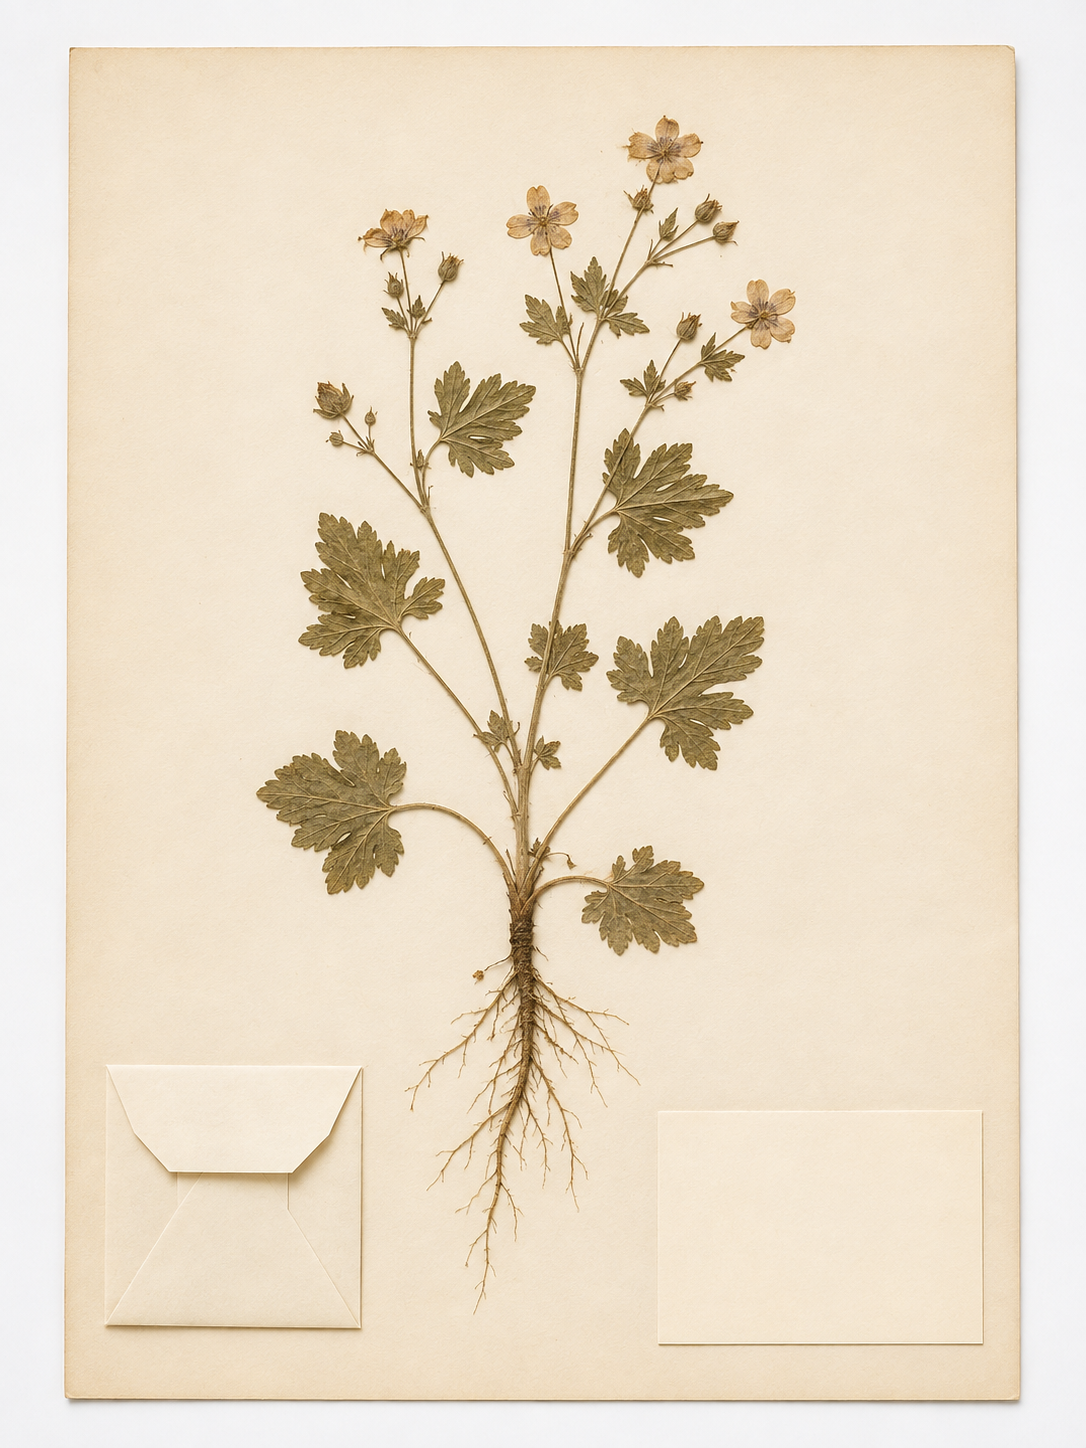
\includegraphics[width=0.5\linewidth]{images/book3/ai/b3-29-herbarium-sheet.png}

{\small ورقة معشبة: عينة مكبوسة معنونة من \omterm{def:b1:classifying-biodiversity:species}{النوع}
الذي يصلح نمطًا لاسم نبات وشاهدًا دائمًا
على أين وُجد \omterm{def:b1:classifying-biodiversity:species}{النوع} ومتى.}
\end{omfigure}

\section{إعادة بناء القرابات}

\begin{definition}[علم التصنيف والشجرة النشوئية والتصنيف التفرعي]\label{def:b1:classifying-biodiversity:systematics}
\index{علم التصنيف}\index{شجرة نشوئية}\index{تصنيف تفرعي}\index{فرع حيوي}
\emph{علم التصنيف} هو دراسة تنوع \omterm{def:b1:organism-environment:organism}{الكائنات} وما
بينها من قرابات؛ و\emph{الشجرة النشوئية} هي شجرة تلك
القرابات، أي فرضية عن ترتيب انشطار السلالات.
و\emph{التصنيف المظهري} يجمع \omterm{def:b1:organism-environment:organism}{الكائنات} بالتشابه الكلي، ويعدّ كل
الصفات بالتساوي؛ و\emph{التصنيف التفرعي} يجمعها بالصفات المشتقة
المشتركة وحدها، حتى تكون كل مجموعة \emph{فرعًا حيويًا} --- أي سلفًا
وكل نسله. والتصنيف الحديث يهدف إلى أن تكون كل \omterm{def:b1:classifying-biodiversity:nomenclature}{وحدة
تصنيفية} مسمّاة فرعًا حيويًا.
\end{definition}

\begin{definition}[الصفات: التماثل والتشابه العارض والقطبية]\label{def:b1:classifying-biodiversity:characters}
\index{تماثل}\index{تشابه عارض}\index{صفة مشتقة مشتركة}\index{مجموعة خارجية}
\emph{الصفة} أي سمة موروثة لها حالتان أو أكثر
(\emph{حالات}) (طرف حاضر أو غائب؛ \omterm{def:b1:nucleic-acids:nucleotide}{قاعدة} معطاة في \omterm{def:b1:genomes:gene}{مورّثة} A أو C أو G
أو T). وصفتا كائنين \emph{متماثلتان} حين تُورَّثان
من سلف مشترك، و\emph{متشابهتان عرضًا} حين تتشابهان بالتقارب
أو بالارتداد (أجنحة الطيور والخفافيش؛ والأجسام الانسيابية عند
الدلافين والقروش). وحالة الصفة \emph{سلفية}
(بليسيومورفية) إن كانت حاضرة في سلف المجموعة، و\emph{مشتقة}
(أبومورفية) إن نشأت داخل المجموعة؛ والحالات المشتقة المشتركة
في \omterm{def:b1:classifying-biodiversity:systematics}{فرع حيوي}، وهي \emph{صفاته المشتقة المشتركة}، هي الشاهد الوحيد عليه.
وتُحدَّد القطبية بالمقارنة مع \emph{مجموعة خارجية}، وهي \omterm{def:b1:classifying-biodiversity:nomenclature}{وحدة تصنيفية}
معلوم وقوعها خارج المجموعة المدروسة: فتُؤخذ الحالة التي تظهرها
سلفيةً.
\end{definition}

\begin{definition}[الأحادية العرق وشبه العرقية وتعدد العرق]\label{def:b1:classifying-biodiversity:monophyly}
\index{أحادية العرق}\index{شبه عرقية}\index{تعدد العرق}
المجموعة \emph{أحادية العرق} (أي \omterm{def:b1:classifying-biodiversity:systematics}{فرع حيوي}) إن ضمّت سلفًا
وكل نسله؛ و\emph{شبه عرقية} إن ضمّت
سلفًا وبعض نسله فقط («الزواحف» التي
تستبعد الطيور المنحدرة منها؛ و«الأسماك» التي تستبعد
رباعيات الأطراف؛ و«اللافقاريات»)؛ و\emph{متعددة العرق} إن جمعت
نسل أسلاف مختلفين بصفة متقاربة («الحيوانات
ذوات الدم الحار»، أي الطيور والثدييات؛ و«الطحالب»). والمجموعات شبه العرقية
أوصاف مفيدة لدرجات التنظيم لكنها ليست
فروعًا حيوية ولم تعد تُعطى أسماء رسمية.
\end{definition}

\begin{omfigure}
\begin{tikzpicture}[font=\footnotesize, line cap=round, >=Stealth]
  % tree: lamprey, shark, trout, lungfish, frog, lizard, bird, mammal
  \coordinate (r) at (6.5,-1.2);
  \draw[thick] (r) -- (6.5,-0.2);
  \draw[thick] (6.5,-0.2) -- (0.5,-0.2) -- (0.5,4.6); \node[anchor=south, rotate=60, anchor=west] at (0.5,4.6) {جلكى};
  \draw[thick] (6.5,-0.2) -- (6.5,0.6) -- (2.2,0.6) -- (2.2,4.6); \node[rotate=60, anchor=west] at (2.2,4.6) {قرش};
  \draw[thick] (6.5,0.6) -- (6.5,1.3) -- (3.8,1.3) -- (3.8,4.6); \node[rotate=60, anchor=west] at (3.8,4.6) {سلمون مرقط};
  \draw[thick] (6.5,1.3) -- (6.5,2.0) -- (5.2,2.0) -- (5.2,4.6); \node[rotate=60, anchor=west] at (5.2,4.6) {سمكة رئوية};
  \draw[thick] (6.5,2.0) -- (6.5,2.7) -- (6.6,2.7) -- (6.6,4.6); \node[rotate=60, anchor=west] at (6.6,4.6) {ضفدع};
  \draw[thick] (6.5,2.7) -- (8.7,2.7) -- (8.7,3.3);
  \draw[thick] (8.7,3.3) -- (8.0,3.3) -- (8.0,4.6); \node[rotate=60, anchor=west] at (8.0,4.6) {ثدييّ};
  \draw[thick] (8.7,3.3) -- (9.7,3.3) -- (9.7,3.9);
  \draw[thick] (9.7,3.9) -- (9.3,3.9) -- (9.3,4.6); \node[rotate=60, anchor=west] at (9.3,4.6) {سحلية};
  \draw[thick] (9.7,3.9) -- (10.6,3.9) -- (10.6,4.6); \node[rotate=60, anchor=west] at (10.6,4.6) {طائر};
  % groupings
  \draw[very thick, omDef, rounded corners=6pt] (7.6,3.05) rectangle (11.0,5.9); \node[omDef!80!black, anchor=south west] at (7.65,5.9) {السلويات: أحادية العرق};
  \draw[very thick, omThm, dashed, rounded corners=6pt] (9.0,3.6) -- (9.0,5.8) -- (10.15,5.8) -- (10.15,3.6) -- cycle; \node[omThm!80!black, anchor=west, align=left] at (11.1,4.8) {«الزواحف»\\ بلا الطيور:\\ شبه عرقية};
  \draw[very thick, omProp!80!black, dotted, rounded corners=6pt] (7.7,6.35) -- (7.7,6.8) -- (11.0,6.8) -- (11.0,6.35); \node[omProp!80!black, anchor=south] at (9.35,6.85) {«ذوات الدم الحار» (ثدييّ $+$ طائر): متعددة العرق};
  \draw[very thick, gray, dashed, rounded corners=6pt] (1.8,4.3) -- (1.8,5.75) -- (5.7,5.75) -- (5.7,4.3); \node[gray, anchor=south] at (3.75,5.9) {«الأسماك» بلا رباعيات الأطراف: شبه عرقية};
  % synapomorphies
  \node[font=\scriptsize, anchor=east] at (6.4,0.2) {فكوك}; \draw[thick] (6.35,0.2) -- (6.65,0.2);
  \node[font=\scriptsize, anchor=east] at (6.4,0.95) {هيكل عظمي}; \draw[thick] (6.35,0.95) -- (6.65,0.95);
  \node[font=\scriptsize, anchor=east] at (6.4,1.65) {رئات}; \draw[thick] (6.35,1.65) -- (6.65,1.65);
  \node[font=\scriptsize, anchor=east] at (6.4,2.35) {أربعة أطراف}; \draw[thick] (6.35,2.35) -- (6.65,2.35);
  \node[font=\scriptsize, anchor=west] at (8.8,2.82) {بيضة سلوية}; \draw[thick] (8.55,2.82) -- (8.85,2.82);
\end{tikzpicture}

{\small مخطط تفرعي لثمانية فقاريات وعليه الصفات المشتقة
المشتركة على الفروع. فالفروع الحيوية \omterm{def:b1:classifying-biodiversity:monophyly}{أحادية العرق}؛ و«الأسماك»
و«الزواحف» درجتان شبه عرقيتين؛ و«الحيوانات ذوات الدم الحار» تجميع
متعدد العرق بصفة متقاربة.}
\end{omfigure}

\begin{definition}[الاقتصاد]\label{def:b1:classifying-biodiversity:parsimony}
\index{اقتصاد}\index{طول الشجرة}
من بين كل الشجرات التي قد تربط مجموعة من الوحدات التصنيفية، تكون
\emph{الأكثر اقتصادًا} هي التي تقتضي أقل عدد من التغيرات
التطورية في حالات الصفات --- أي أصغر \emph{طول شجرة}، وهو
مجموع أقل عدد من التغيرات يحتاج إليه كل صفة على
تلك الشجرة. والصفة التي تلائم الشجرة بتغير واحد
متسقة معها؛ والتي تحتاج إلى تغيرين أو أكثر \omterm{def:b1:classifying-biodiversity:characters}{تشابه عارض} على
تلك الشجرة. والاقتصاد ليس دعوى بأن التطور مقتصد؛ بل
هو \omterm{def:b1:nucleic-acids:nucleotide}{قاعدة} بأن الفرضية لا ينبغي أن تكثر التقاربات
فوق ما تفرضه المعطيات.
\end{definition}

\begin{method}[بناء مخطط تفرعي من مصفوفة صفات]\label{met:b1:classifying-biodiversity:cladogram}
\begin{enumerate}
  \item اختر الوحدات التصنيفية \omterm{def:b1:classifying-biodiversity:characters}{ومجموعة خارجية}؛ واسرد الصفات بحالاتها،
        مرمّزًا حالة \omterm{def:b1:classifying-biodiversity:characters}{المجموعة الخارجية} 0 (سلفية)
        والحالة المشتقة 1.
  \item اجمع الوحدات بالحالات المشتقة المشتركة، ابتداءً من
        الصفة التي يتقاسمها أكثر الوحدات (\omterm{def:b1:classifying-biodiversity:systematics}{الفرع الحيوي} الأعمق)
        وتعشيشًا إلى الداخل؛ وكل 1 تتقاسمه مجموعة من الوحدات
        صفةٌ مشتقة مشتركة مرشحة لتلك المجموعة.
  \item وحيث تتعارض الصفات (فلا تستطيع مجموعتان أن تكونا
        فرعين حيويين معًا)، ارسم كل شجرة بديلة وعُدّ طولها:
        أي لكل صفة، أقل عدد من التغيرات يضع حالاتها
        على الشجرة.
  \item أبقِ أقصر شجرة؛ والصفات التي احتاجت إلى تغيرات
        زائدة عليها هي التشابهات العارضة. وإن تعادلت شجرتان فإن
        المعطيات لا تحسم ويلزم صفات أكثر.
  \item اقرأ الشجرة: سمِّ الفروع الحيوية، ولاحظ أي المجموعات التقليدية
        \omterm{def:b1:classifying-biodiversity:monophyly}{شبه عرقية}، وتحقق من توافقها مع معطيات مستقلة
        (تسلسلات جزيئية، وأحافير).
\end{enumerate}
\end{method}

\begin{example}[شجرتان، معدودتان]\label{ex:b1:classifying-biodiversity:count}
أربع وحدات: سحلية، وطائر، وثدييّ، وضفدع (\omterm{def:b1:classifying-biodiversity:characters}{مجموعة خارجية}). والصفات:
البيضة السلوية (السحلية والطائر والثدييّ: 1)، والجمجمة ثنائية القوس (السحلية
والطائر)، والتدفئة الداخلية (الطائر والثدييّ). فالشجرة A، (سحلية، طائر) ثم ثدييّ:
البيضة تغير واحد، والجمجمة 1، والتدفئة الداخلية 2 (إذ تنشأ مرتين) --- فالطول 4.
والشجرة B، (طائر، ثدييّ) ثم سحلية: البيضة 1، والتدفئة الداخلية 1، والجمجمة 2 ---
فالطول 4. أي تعادل؛ فأضف الريش وحراشف الساق
والحراشف البشروية (السحلية والطائر): فيصير \omterm{def:b1:classifying-biodiversity:parsimony}{طول الشجرة} A خمسة \omterm{def:b1:classifying-biodiversity:parsimony}{وطول الشجرة} B ستة. فالشجرة A
مفضَّلة، والتدفئة الداخلية \omterm{def:b1:classifying-biodiversity:characters}{تشابه عارض}: فقد تطورت مرتين.
\end{example}

\begin{omfigure}
\begin{tikzpicture}[font=\footnotesize, line cap=round]
  \begin{scope}
    \draw[thick] (2.0,0) -- (2.0,0.8);
    \draw[thick] (2.0,0.8) -- (0,0.8) -- (0,3.0); \node[anchor=south] at (0,3.0) {ضفدع};
    \draw[thick] (2.0,0.8) -- (2.0,1.6) -- (1.2,1.6) -- (1.2,3.0); \node[anchor=south] at (1.2,3.0) {ثدييّ};
    \draw[thick] (2.0,1.6) -- (3.0,1.6) -- (3.0,2.3);
    \draw[thick] (3.0,2.3) -- (2.4,2.3) -- (2.4,3.0); \node[anchor=south] at (2.4,3.0) {سحلية};
    \draw[thick] (3.0,2.3) -- (3.6,2.3) -- (3.6,3.0); \node[anchor=south] at (3.6,3.0) {طائر};
    \draw[very thick, omDef] (1.85,1.2) -- (2.15,1.2); \node[anchor=east, font=\scriptsize, omDef!80!black] at (1.8,1.2) {بيضة};
    \draw[very thick, omDef] (2.85,1.95) -- (3.15,1.95); \node[anchor=west, font=\scriptsize, omDef!80!black] at (3.2,1.95) {جمجمة وحراشف};
    \draw[very thick, omThm] (1.05,2.5) -- (1.35,2.5); \node[anchor=east, font=\scriptsize, omThm] at (1.0,2.5) {تدفئة};
    \draw[very thick, omThm] (3.45,2.65) -- (3.75,2.65); \node[anchor=west, font=\scriptsize, omThm] at (3.8,2.65) {تدفئة};
    \node[anchor=north, align=center] at (1.9,-0.2) {الشجرة A: الطول 5\\ (التدفئة الداخلية مرتين)};
  \end{scope}
  \begin{scope}[xshift=7.4cm]
    \draw[thick] (2.0,0) -- (2.0,0.8);
    \draw[thick] (2.0,0.8) -- (0,0.8) -- (0,3.0); \node[anchor=south] at (0,3.0) {ضفدع};
    \draw[thick] (2.0,0.8) -- (2.0,1.6) -- (1.2,1.6) -- (1.2,3.0); \node[anchor=south] at (1.2,3.0) {سحلية};
    \draw[thick] (2.0,1.6) -- (3.0,1.6) -- (3.0,2.3);
    \draw[thick] (3.0,2.3) -- (2.4,2.3) -- (2.4,3.0); \node[anchor=south] at (2.4,3.0) {ثدييّ};
    \draw[thick] (3.0,2.3) -- (3.6,2.3) -- (3.6,3.0); \node[anchor=south] at (3.6,3.0) {طائر};
    \draw[very thick, omDef] (1.85,1.2) -- (2.15,1.2); \node[anchor=east, font=\scriptsize, omDef!80!black] at (1.8,1.2) {بيضة};
    \draw[very thick, omDef] (2.85,1.95) -- (3.15,1.95); \node[anchor=west, font=\scriptsize, omDef!80!black] at (3.2,1.95) {تدفئة};
    \draw[very thick, omThm] (1.05,2.5) -- (1.35,2.5); \node[anchor=east, font=\scriptsize, omThm, align=right] at (1.0,2.5) {جمجمة\\ وحراشف};
    \draw[very thick, omThm] (3.45,2.65) -- (3.75,2.65); \node[anchor=west, font=\scriptsize, omThm, align=left] at (3.8,2.65) {جمجمة\\ وحراشف};
    \node[anchor=north, align=center] at (1.9,-0.2) {الشجرة B: الطول 6\\ (الجمجمة والحراشف مرتين)};
  \end{scope}
\end{tikzpicture}

{\small \omterm{def:b1:classifying-biodiversity:parsimony}{الاقتصاد} يحكم بين شجرتين بعدّ التغيرات التي
تقتضيها كل واحدة. فالشجرة A تحتاج إلى \omterm{def:b1:classifying-biodiversity:characters}{تشابه عارض} واحد (التدفئة الداخلية تنشأ مرتين)؛
والشجرة B تحتاج إلى اثنين؛ فتُبقى الشجرة A.}
\end{omfigure}

\begin{remark}[الصفات الجزيئية]\label{rem:b1:classifying-biodiversity:molecular}
تمدّ تسلسلة \omterm{def:b1:genomes:gene}{مورّثة} بمئات الصفات دفعة واحدة، كل موضع فيها
صفة لها أربع حالات، قابلة للمقارنة عبر \omterm{def:b1:organism-environment:organism}{كائنات} لا تشترك
في أي سمة مرئية --- بكتيريا وبلوطة. فتُصفّ التسلسلات، وتُقارن
المواضع المتماثلة، وتُبنى الشجرات \omterm{def:b1:classifying-biodiversity:parsimony}{بالاقتصاد} أو بطرائق
إحصائية تنمذج معدل الاستبدال؛ والساعة
الجزيئية، وهي المعدل الذي تتراكم به الفروق المحايدة،
تؤرخ الانشطارات. وتُتناول الطرائق، ومزالق الفروع الطويلة
والمعدلات غير المتساوية، في كتاب السنة الثانية.
\end{remark}

\section{شجرة الحياة}

\begin{proposition}[ثلاثة مجالات]\label{prop:b1:classifying-biodiversity:domains}
\index{مجال}\index{Archaea}\index{Bacteria}\index{Eukarya}
تنقسم الحياة إلى ثلاثة مجالات: \emph{Bacteria} و\emph{Archaea} و
\emph{Eukarya}. وBacteria وArchaea كلاهما بدائي \omterm{def:b1:eukaryotic-cell:nucleus}{النواة} في تنظيم
\omterm{def:b1:cell-unit-of-life:cell}{الخلية} (\cref{ch:b1:cell-unit-of-life}) لكنهما يختلفان في
دهون أغشيتهما وجدرهما الخلوية وبوليميرازات \omterm{def:b1:nucleic-acids:chain}{RNA} فيهما وريبوزوماتهما؛
وآلة الاستنساخ والترجمة في Archaea أقرب إلى آلة \omterm{def:b1:cell-unit-of-life:prokeuk}{حقيقيات النواة}
منها إلى آلة البكتيريا، وقد نشأت \omterm{def:b1:cell-unit-of-life:prokeuk}{الخلية حقيقية النواة}
من سلالة أركية اكتسبت بكتيريا متقدرةً لها
(\cref{ch:b1:eukaryotic-cell}). وداخل Eukarya حلّ محل
الممالك القديمة --- الحيوانات والنباتات والفطريات وبقية «طلائعية» ---
حفنة من السلالات الكبرى، ليست الحيوانات
والفطريات والنباتات البرية منها إلا ثلاثة أغصان صغيرة،
و«الطلائعيات» خليط شبه عرقي من كل ما عداها.
\end{proposition}
\begin{proof}[شواهد]
قارن ويزي وفوكس (1977) تسلسلة \omterm{def:b1:nucleic-acids:rnas}{RNA الريبوزومي} في الوحدة
الصغيرة --- وهو جزيء تملكه كل \omterm{def:b1:cell-unit-of-life:cell}{خلية}، بالوظيفة نفسها وقابل
للصفّ عبر الحياة كلها --- بين البكتيريا ومولّدات الميثان و
\omterm{def:b1:cell-unit-of-life:prokeuk}{حقيقيات النواة}، فوجدا أن مولّدات الميثان تختلف عن سائر
البكتيريا بقدر اختلاف أي منهما عن \omterm{def:b1:cell-unit-of-life:prokeuk}{حقيقيات النواة}. فكانت
\omterm{def:b1:cell-unit-of-life:prokeuk}{بدائيات النواة} مجموعتين لا واحدة؛ وقد أكدت الشجرة المرسومة من هذه
\omterm{def:b1:genomes:gene}{المورّثة} الواحدة مورثوماتٌ كاملة وكيمياء حيوية متميزة
لمجال Archaea (دهون مرتبطة بالإيثر، ولا \omterm{def:b1:carbohydrates:polysaccharide}{ببتيدوغليكان}).
\end{proof}

\begin{omfigure}
\begin{tikzpicture}[font=\footnotesize, line cap=round]
  \coordinate (root) at (5.0,0);
  \draw[very thick] (root) -- (5.0,1.0);
  \draw[very thick, omExo!80!black] (5.0,1.0) -- (1.6,1.0) -- (1.6,2.4);
  \draw[very thick, omExo!80!black] (1.6,2.4) -- (0.4,2.4) -- (0.4,3.6); \draw[very thick, omExo!80!black] (1.6,2.4) -- (1.6,3.6); \draw[very thick, omExo!80!black] (1.6,2.4) -- (2.8,2.4) -- (2.8,3.6);
  \node[anchor=south, rotate=60, anchor=west] at (0.4,3.6) {بكتيريا بروتينية}; \node[rotate=60, anchor=west] at (1.6,3.6) {بكتيريا زرقاء}; \node[rotate=60, anchor=west] at (2.8,3.6) {إيجابيات الغرام};
  \node[omExo!80!black, font=\small, anchor=north] at (1.6,0.9) {Bacteria};
  \draw[very thick] (5.0,1.0) -- (7.6,1.0) -- (7.6,1.7);
  \draw[very thick, omProp!80!black] (7.6,1.7) -- (5.8,1.7) -- (5.8,2.4);
  \draw[very thick, omProp!80!black] (5.8,2.4) -- (5.0,2.4) -- (5.0,3.6); \draw[very thick, omProp!80!black] (5.8,2.4) -- (6.6,2.4) -- (6.6,3.6);
  \node[rotate=60, anchor=west] at (5.0,3.6) {مولّدات الميثان}; \node[rotate=60, anchor=west] at (6.6,3.6) {محبات الملوحة};
  \node[omProp!80!black, font=\small, anchor=north] at (5.8,1.6) {Archaea};
  \draw[very thick, omDef] (7.6,1.7) -- (9.6,1.7) -- (9.6,2.4);
  \draw[very thick, omDef] (9.6,2.4) -- (8.0,2.4) -- (8.0,3.6); \draw[very thick, omDef] (9.6,2.4) -- (9.0,2.4) -- (9.0,3.6); \draw[very thick, omDef] (9.6,2.4) -- (10.0,2.4) -- (10.0,3.6); \draw[very thick, omDef] (9.6,2.4) -- (11.0,2.4) -- (11.0,3.6);
  \node[rotate=60, anchor=west] at (8.0,3.6) {نباتات برية وطحالب}; \node[rotate=60, anchor=west] at (9.0,3.6) {فطريات}; \node[rotate=60, anchor=west] at (10.0,3.6) {حيوانات}; \node[rotate=60, anchor=west] at (11.0,3.6) {سلالات طلائعية كثيرة};
  \node[omDef!80!black, font=\small, anchor=north] at (9.6,1.6) {Eukarya};
  \draw[->, thick, gray, dashed] (1.6,2.0) to[out=0, in=180] (9.6,2.1); \node[gray, font=\scriptsize, anchor=west] at (5.2,0.5) {بكتيريا صارت المتقدرة};
  \node[anchor=north] at (5.0,-0.1) {السلف المشترك العام الأخير};
\end{tikzpicture}

{\small المجالات الثلاثة، من \omterm{def:b1:nucleic-acids:rnas}{RNA الريبوزومي}. ومجال Archaea أقرب
أقرباء \omterm{def:b1:cell-unit-of-life:prokeuk}{حقيقيات النواة}، \omterm{def:b1:cell-unit-of-life:prokeuk}{والخلية حقيقية النواة} اندماج:
مضيف أركي \omterm{def:b1:eukaryotic-cell:mitochondrion}{بمتقدرة} بكتيرية (وفي النباتات
والطحالب، شريك بكتيري ثانٍ هو \omterm{def:b1:photosynthesis:chloroplast}{البلاستيدة الخضراء}).}
\end{omfigure}

\begin{omfigure}
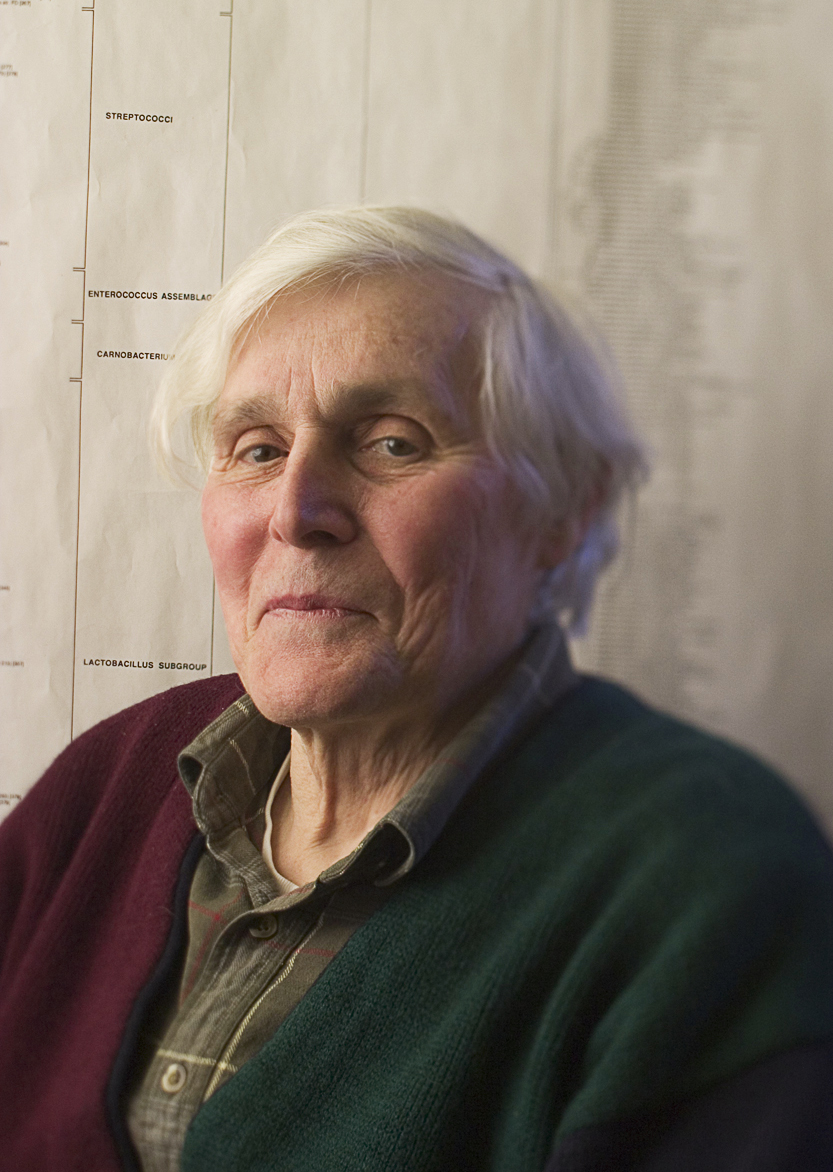
\includegraphics[width=0.34\linewidth]{images/book3/woese.jpg}

{\small كارل ويزي (Carl Woese) (1928--2012)، أمام شجرة من \omterm{def:b1:nucleic-acids:rnas}{RNA الريبوزومي}
للبكتيريا. وقد كشفت مقارنته لهذا الجزيء الواحد عبر الحياة كلها
Archaea وأعطت شجرة الحياة مجالاتها الثلاثة.}
\end{omfigure}

\begin{proposition}[سلالات حقيقيات النواة الكبرى]\label{prop:b1:classifying-biodiversity:eukaryotes}
تقع \omterm{def:b1:cell-unit-of-life:prokeuk}{حقيقيات النواة} في بضع مجموعات كبرى: \emph{Opisthokonta}
(الحيوانات والفطريات وأقرباؤها وحيدة \omterm{def:b1:cell-unit-of-life:cell}{الخلية}، وخلاياها تسبح
بسوط خلفي واحد)؛ و\emph{Archaeplastida} (النباتات البرية،
والطحالب الخضراء والحمراء، \omterm{def:b1:photosynthesis:chloroplast}{بالبلاستيدة الخضراء} الأولية)؛ و
\emph{Amoebozoa}؛ و\emph{Excavata} (سوطيات مثل
\emph{Trypanosoma} و\emph{Euglena})؛ ومجموعة \emph{SAR}
(السترامينوبيلات مثل الدياتومات والطحالب البنية؛ والحويصليات مثل
الهدبيات والسوطيات الدوّارة \omterm{def:b1:species-interactions:symbiosis}{وطفيلي} الملاريا؛ والريزاريات مثل
المنخربات والشعاعيات). فالحيوانات والفطريات إذن أقرب
بعضها إلى بعض من قرب أي منها إلى النباتات؛ و«الطحالب» مبعثرة
عبر أربع مجموعات؛ وأغلبية تنوع \omterm{def:b1:cell-unit-of-life:prokeuk}{حقيقيات النواة} المجهرية
تقع خارج الممالك الثلاث ذوات الأسماء الشائعة.
\end{proposition}

\begin{omfigure}
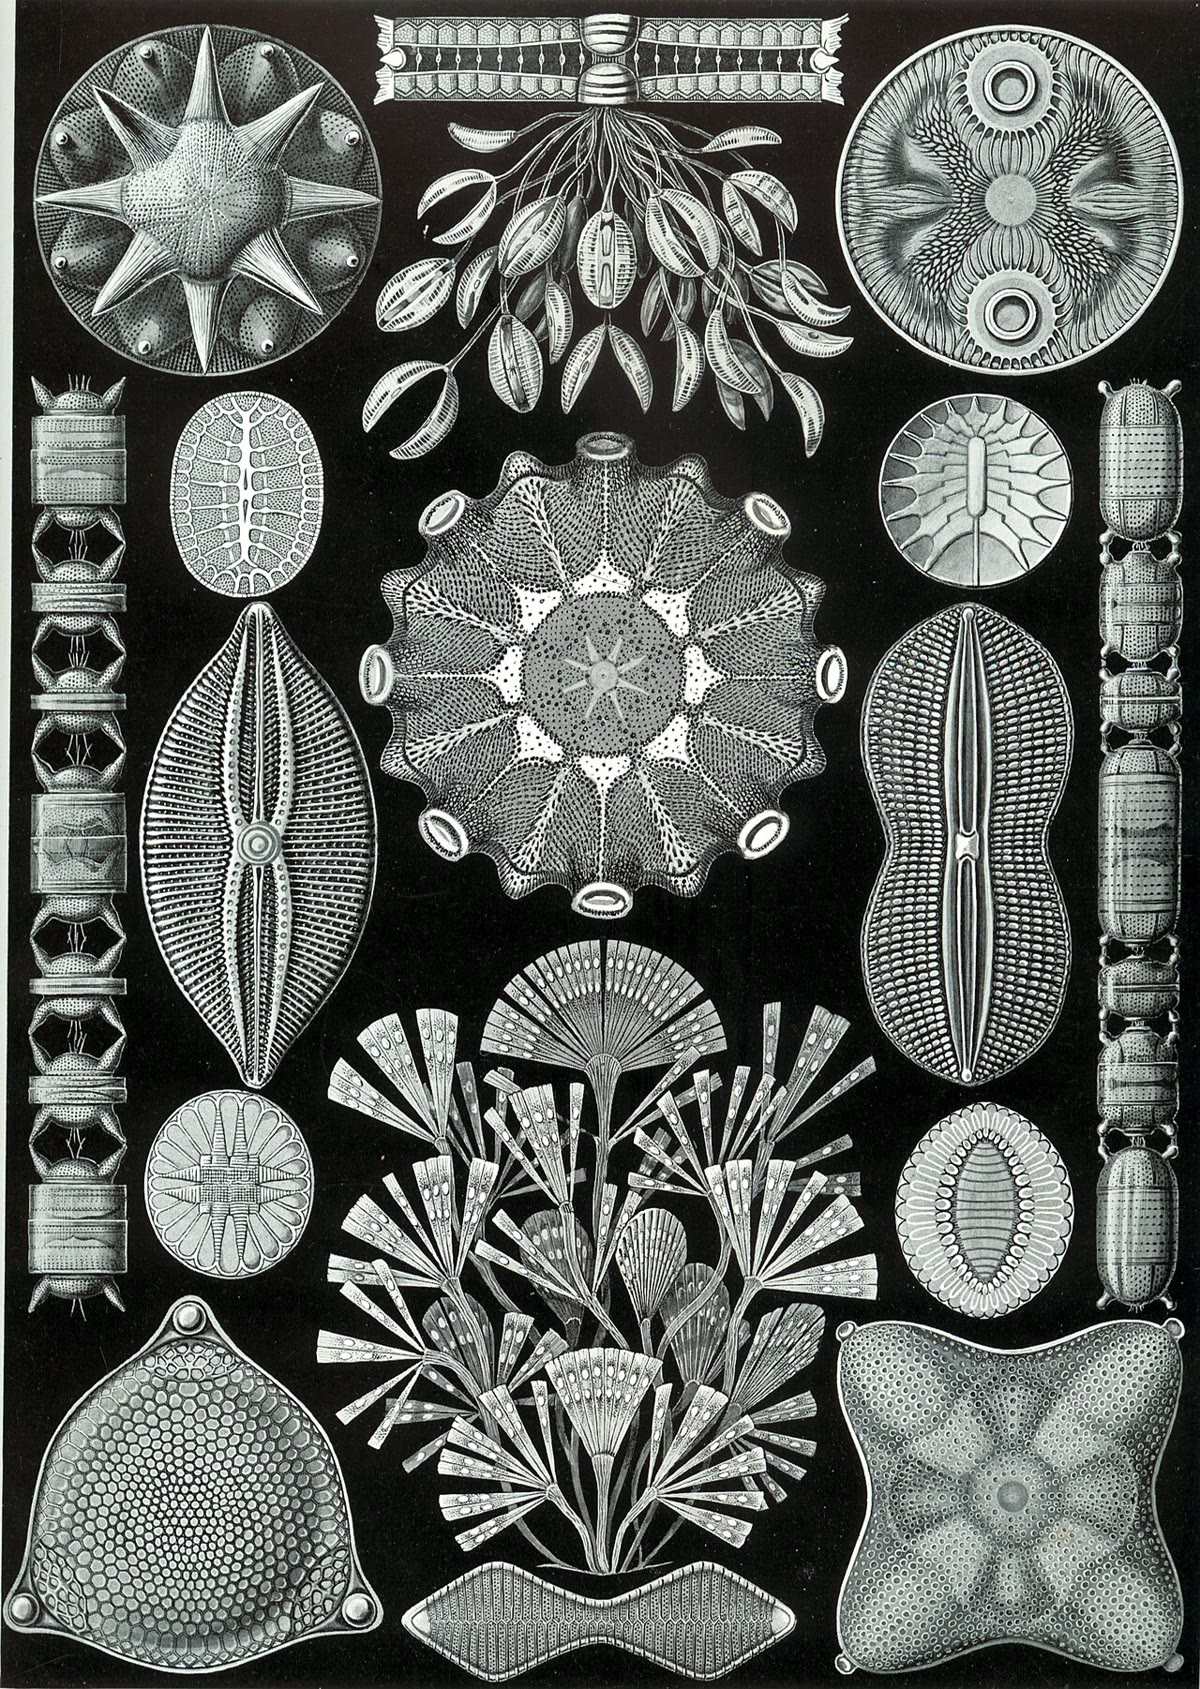
\includegraphics[width=0.36\linewidth]{images/book3/haeckel-diatomea.jpg}\hspace{0.03\linewidth}
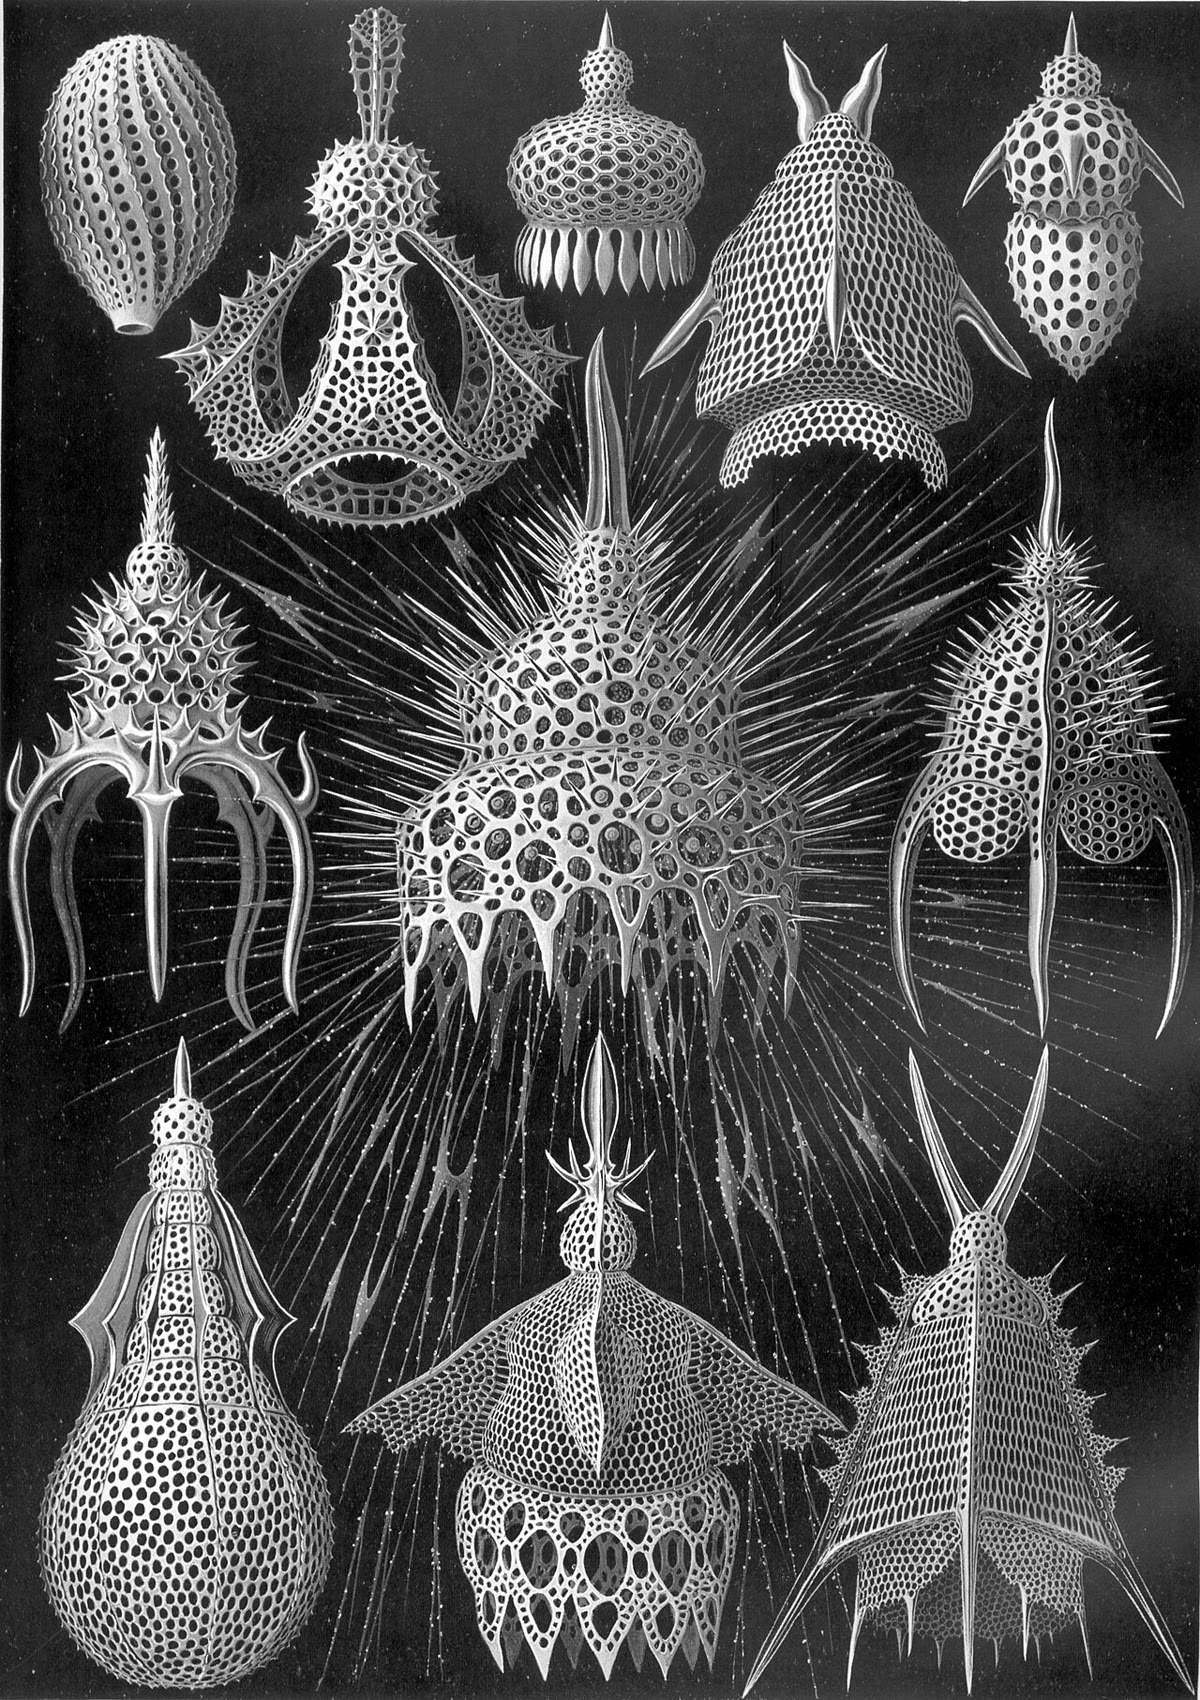
\includegraphics[width=0.36\linewidth]{images/book3/haeckel-cyrtoidea.jpg}

{\small اثنتان من سلالات \omterm{def:b1:cell-unit-of-life:prokeuk}{حقيقيات النواة} التي لا اسم شائع لها، في
لوحات إرنست هيكل (Ernst Haeckel) سنة 1904: الدياتومات (سترامينوبيلات، في أصداف
سيليكية) والشعاعيات (ريزاريات، في هياكل سيليكية). وكل
مجموعة منهما تضم عشرات الآلاف من \omterm{def:b1:classifying-biodiversity:species}{الأنواع}.}
\end{omfigure}

\section{جرد الحياة}

\begin{definition}[التنوع الحيوي]\label{def:b1:classifying-biodiversity:biodiversity}
\index{تنوع حيوي}\index{انقراض}
\emph{التنوع الحيوي} هو تنوع الحياة على كل مستوى: التنوع
الوراثي داخل \omterm{def:b1:classifying-biodiversity:species}{الأنواع}، وعدد \omterm{def:b1:classifying-biodiversity:species}{الأنواع} ووفرتها، و
تنوع المجتمعات \omterm{def:b1:ecosystem-organization:ecosystem}{والنظم البيئية}. وجرده
غير تام: فقد وُصف نحو \num{2} مليون \omterm{def:b1:classifying-biodiversity:species}{نوع}،
منها مليون من الحشرات، و\num{380000} من النباتات، و\num{150000} من الفطريات،
و\num{70000} من الفقاريات، وبضع عشرات الآلاف من كل من الرخويات
والقشريات والطلائعيات \omterm{def:b1:cell-unit-of-life:prokeuk}{وبدائيات النواة}؛ ويُقدَّر عدد \omterm{def:b1:classifying-biodiversity:species}{أنواع} \omterm{def:b1:cell-unit-of-life:prokeuk}{حقيقيات النواة}،
من معدل العثور على وحدات تصنيفية عليا جديدة إلى اليوم،
بنحو \num{9} ملايين، فيكون أكثر \omterm{def:b1:classifying-biodiversity:species}{الأنواع} بلا اسم،
وأكثر تلك صغيرًا أو مداريًا أو كليهما. وقد ظلت \omterm{def:b1:classifying-biodiversity:species}{الأنواع}
\emph{تنقرض} دائمًا --- والمعدل الخلفي، من الأحافير، نحو
\omterm{def:b1:classifying-biodiversity:species}{نوع} واحد لكل مليون في السنة --- والمعدل الحالي، الذي يسوقه
فقد الموائل والاستغلال \omterm{def:b1:classifying-biodiversity:species}{والأنواع} الغازية والمناخ، يُقدَّر
بمئة إلى ألف مثل من ذلك.
\end{definition}

\begin{omfigure}
\begin{tikzpicture}
\begin{axis}[
  xbar, bar width=7pt,
  width=0.82\linewidth, height=6.8cm,
  axis x line=bottom, axis y line=left,
  xmin=0, xmax=1200, xlabel={الأنواع الموصوفة (بالآلاف)},
  xlabel style={font=\small, at={(axis description cs:0.5,-0.12)}, anchor=north},
  symbolic y coords={بكتيريا وأركيات, ثدييات, طيور, أسماك, طلائعيات, رخويات, قشريات, عنكبيات, فطريات, نباتات برية, حشرات},
  ytick=data, tick label style={font=\small},
  enlarge y limits=0.06, xtick={0,200,400,600,800,1000},
  nodes near coords, nodes near coords style={font=\scriptsize, anchor=west},
]
\addplot[fill=omDef!40, draw=omDef] coordinates {(12,بكتيريا وأركيات) (6.5,ثدييات) (11,طيور) (35,أسماك) (60,طلائعيات) (85,رخويات) (70,قشريات) (110,عنكبيات) (150,فطريات) (380,نباتات برية) (1000,حشرات)};
\end{axis}
\end{tikzpicture}

{\small \omterm{def:b1:classifying-biodiversity:species}{الأنواع} الموصوفة بحسب المجموعة، بالآلاف (مقرَّبة). فنصف
كل \omterm{def:b1:classifying-biodiversity:species}{الأنواع} المسمّاة حشرات، \omterm{def:b1:cell-unit-of-life:prokeuk}{وبدائيات النواة} --- وهي أشد \omterm{def:b1:organism-environment:organism}{الكائنات}
تنوعًا بأي مقياس جزيئي --- لها \omterm{def:b1:classifying-biodiversity:species}{أنواع} موصوفة أقل من
الثدييات والطيور معًا.}
\end{omfigure}

\begin{omfigure}
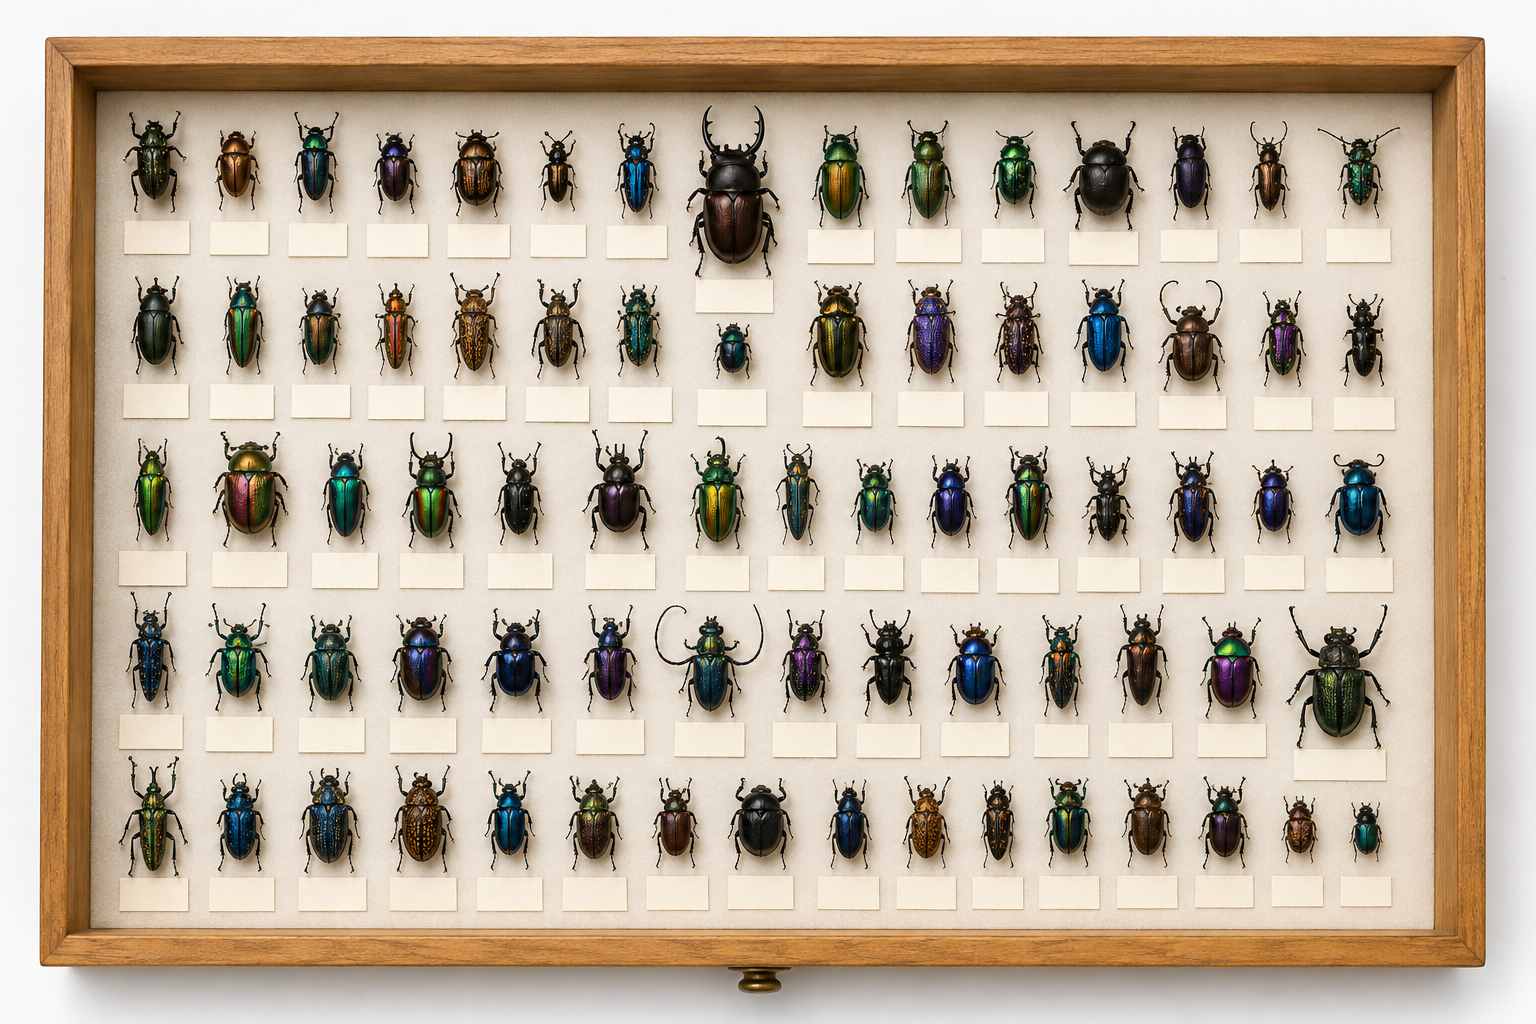
\includegraphics[width=0.56\linewidth]{images/book3/ai/b3-29-beetle-collection.png}

{\small درج متحفي من الخنافس المدبَّسة: فالمجموعة هي
الجرد، ودرج كهذا قد يحمل أنواعًا لم يسمّها أحد
بعد.}
\end{omfigure}

\begin{method}[تقدير كم نوعًا يوجد]\label{met:b1:classifying-biodiversity:estimate}
\begin{enumerate}
  \item عُدّ \omterm{def:b1:classifying-biodiversity:species}{الأنواع} الموصوفة في مجموعة والمعدل الذي ما تزال
        \omterm{def:b1:classifying-biodiversity:species}{الأنواع} الجديدة تُضاف به؛ فإن لم يكن المعدل يتباطأ،
        فالجرد بعيد عن التمام.
  \item استقرِ من مجموعة معلومة جيدًا إلى مجموعة ضعيفة المعرفة
        بنسبة: فإن كانت حيوانات المناطق المعتدلة تحمل نوعي حشرة لكل
        \omterm{def:b1:classifying-biodiversity:species}{نوع} نبات، وفي المدارين \num{250000} نبات، فالمداران
        يحملان نصف مليون حشرة على الأقل.
  \item عيِّن بكثافة مساحة صغيرة (تضبيب تاج شجرة مدارية
        بمبيد حشري، أو تسلسل \omterm{def:b1:nucleic-acids:chain}{DNA} في لتر من ماء البحر)
        وقِس على ذلك من كسر \omterm{def:b1:classifying-biodiversity:species}{الأنواع} الجديدة.
  \item استعمل النمط عبر المراتب: فأعداد الشعب والطوائف
        والرتب والفصائل شبه تامة وترتفع بانتظام
        نحو مستوى \omterm{def:b1:classifying-biodiversity:species}{النوع}؛ واستقراء الانتظام يعطي
        المجموع (نحو \num{8.7} ملايين من \omterm{def:b1:cell-unit-of-life:prokeuk}{حقيقيات النواة}).
  \item اذكر التقدير مع مداه؛ فالجواب الصادق عن
        \omterm{def:b1:cell-unit-of-life:prokeuk}{بدائيات النواة} مدى من عدة رتب من القدر.
\end{enumerate}
\end{method}

\section{تمارين}

\begin{exercise}[$\star$]\label{exo:b1:classifying-biodiversity:1}
اكتب اسم القط المنزلي كتابة صحيحة، وحدّد جنسه ونعته
النوعي، وضعه في فصيلته ورتبته وطائفته وشعبته.
\end{exercise}

\begin{exercise}[$\star$]\label{exo:b1:classifying-biodiversity:2}
عرّف \omterm{def:b1:classifying-biodiversity:characters}{التماثل} \omterm{def:b1:classifying-biodiversity:characters}{والتشابه العارض} بمثال على كل منهما، وقل أيهما
شاهد على \omterm{def:b1:classifying-biodiversity:systematics}{فرع حيوي}.
\end{exercise}

\begin{exercise}[$\star$]\label{exo:b1:classifying-biodiversity:3}
اذكر هل «الأسماك» و«الطيور» و«الحيوانات ذوات الدم الحار»
\omterm{def:b1:classifying-biodiversity:monophyly}{أحادية العرق} أم \omterm{def:b1:classifying-biodiversity:monophyly}{شبه عرقية} أم متعددة العرق، مع السبب.
\end{exercise}

\begin{exercise}[$\star$]\label{exo:b1:classifying-biodiversity:4}
سمِّ المجالات الثلاثة وأعطِ سمتين تفصلان
Archaea عن Bacteria.
\end{exercise}

\begin{exercise}[$\star\star$]\label{exo:b1:classifying-biodiversity:5}
لماذا لا يمكن تطبيق \omterm{def:b1:classifying-biodiversity:species}{مفهوم النوع البيولوجي} على البكتيريا أو
على الأحافير، وماذا يُستعمل بدله؟
\end{exercise}

\begin{exercise}[$\star\star$]\label{exo:b1:classifying-biodiversity:6}
ثلاث وحدات X وY وZ \omterm{def:b1:classifying-biodiversity:characters}{ومجموعة خارجية}. والصفة 1 مشتقة في X وY؛
والصفة 2 في Y وZ؛ والصفة 3 في X وY؛ والصفة 4 في X و
Y. ارسم الشجرتين الممكنتين، واحسب طوليهما، وأعطِ
الأكثر اقتصادًا وتشابهها العارض.
\end{exercise}

\begin{exercise}[$\star\star$]\label{exo:b1:classifying-biodiversity:7}
لماذا تلزم \omterm{def:b1:classifying-biodiversity:characters}{مجموعة خارجية} لبناء مخطط تفرعي، وماذا يفسد
إن كانت \omterm{def:b1:classifying-biodiversity:characters}{المجموعة الخارجية} المختارة تنتمي في الحقيقة إلى داخل المجموعة؟
\end{exercise}

\begin{exercise}[$\star\star$]\label{exo:b1:classifying-biodiversity:8}
فسّر لماذا تُعدّ الحيوانات والفطريات أقرب قرابة من
الحيوانات والنباتات، وأي صفة تتقاسمها Opisthokonta.
\end{exercise}

\begin{exercise}[$\star\star$]\label{exo:b1:classifying-biodiversity:9}
وجد ويزي أن مولّدات الميثان تختلف عن سائر البكتيريا بقدر
اختلافها عن \omterm{def:b1:cell-unit-of-life:prokeuk}{حقيقيات النواة}. فلماذا برر هذا مجالًا جديدًا لا مملكة
جديدة داخل البكتيريا؟
\end{exercise}

\begin{exercise}[$\star\star\star$]\label{exo:b1:classifying-biodiversity:10}
تاج شجرة مدارية يُضبَّب بمبيد حشري يعطي 1200 \omterm{def:b1:classifying-biodiversity:species}{نوع}
خنفساء، منها \qty{20}{\%} خاصة بذلك \omterm{def:b1:classifying-biodiversity:species}{النوع} من الشجر؛
والخنافس \qty{40}{\%} من حشرات التاج، والتاج
يحمل ثلثي حشرات الشجرة؛ وثمة \num{50000}
\omterm{def:b1:classifying-biodiversity:species}{نوع} شجر مداري. قدّر عدد \omterm{def:b1:classifying-biodiversity:species}{أنواع} الحشرات المدارية
واسرد الفرضيات.
\end{exercise}

\begin{exercise}[$\star\star\star$]\label{exo:b1:classifying-biodiversity:11}
يُوصف \omterm{def:b1:classifying-biodiversity:species}{نوع} من عينة متحفية واحدة؛ ثم تُوجد \omterm{def:b1:populations:population}{جمهرات}
حية تختلف عنها قليلًا. فسّر دور \omterm{def:b1:classifying-biodiversity:nomenclature}{العينة النمطية} في
تقرير ما ينطبق عليه الاسم، ولماذا تهمّ الأولوية.
\end{exercise}

\begin{exercise}[$\star\star\star$]\label{exo:b1:classifying-biodiversity:12}
«\omterm{def:b1:classifying-biodiversity:parsimony}{الاقتصاد} يفترض أن التطور يسلك أقصر طريق.» ناقش:
ماذا يفترض \omterm{def:b1:classifying-biodiversity:parsimony}{الاقتصاد} فعلًا، ومتى يخفق (التقارب، والسلالات سريعة
التطور)، وكيف تُستعمل المعطيات الجزيئية والأحافير في تدقيق
شجرة.
\end{exercise}

\section{مسألة: ثمانية فقاريات وشجرة}

\begin{problem}[{مسألة نهاية الأسبوع --- مصفوفة صفات لثمانية
فقاريات، ومخططها التفرعي مبنيًا باليد، وشجرتان متنافستان تُقيَّمان
بالاقتصاد، والمجموعات التقليدية تُختبر لأحادية العرق، وتقدير
لعدد الأنواع، وختامًا الشجرة الأكثر اقتصادًا
وطولها}]
\label{pb:b1:classifying-biodiversity:1}
تسجّل المصفوفة عشر صفات (1 = الحالة المشتقة حاضرة) لكل من
الجلكى (\omterm{def:b1:classifying-biodiversity:characters}{مجموعة خارجية})، وقرش، وسلمون مرقط، وسمكة رئوية، وضفدع، وسحلية،
وفأر، وحمامة.

\begin{center}
\footnotesize
\begin{tabular}{l*{10}{c}}
\hline
 & 1 & 2 & 3 & 4 & 5 & 6 & 7 & 8 & 9 & 10 \\
 & \rotatebox{90}{فكوك} & \rotatebox{90}{هيكل عظمي} & \rotatebox{90}{رئات} & \rotatebox{90}{أربعة أطراف} & \rotatebox{90}{بيضة سلوية} & \rotatebox{90}{شعر} & \rotatebox{90}{ريش} & \rotatebox{90}{جمجمة ثنائية القوس} & \rotatebox{90}{تدفئة داخلية} & \rotatebox{90}{حراشف كيراتينية} \\
\hline
جلكى & 0 & 0 & 0 & 0 & 0 & 0 & 0 & 0 & 0 & 0 \\
قرش & 1 & 0 & 0 & 0 & 0 & 0 & 0 & 0 & 0 & 0 \\
سلمون مرقط & 1 & 1 & 0 & 0 & 0 & 0 & 0 & 0 & 0 & 0 \\
سمكة رئوية & 1 & 1 & 1 & 0 & 0 & 0 & 0 & 0 & 0 & 0 \\
ضفدع & 1 & 1 & 1 & 1 & 0 & 0 & 0 & 0 & 0 & 0 \\
سحلية & 1 & 1 & 1 & 1 & 1 & 0 & 0 & 1 & 0 & 1 \\
فأر & 1 & 1 & 1 & 1 & 1 & 1 & 0 & 0 & 1 & 0 \\
حمامة & 1 & 1 & 1 & 1 & 1 & 0 & 1 & 1 & 1 & 1 \\
\hline
\end{tabular}
\end{center}

\medskip
\noindent\textbf{الجزء الأول --- قراءة المصفوفة.}
\begin{enumerate}
  \item أي الصفات تتقاسمها كل الوحدات إلا \omterm{def:b1:classifying-biodiversity:characters}{المجموعة الخارجية}؟
        وماذا تقول عن الشجرة؟
  \item اسرد الصفات بترتيب عدد الوحدات التي تتقاسم
        الحالة المشتقة، وقل أي \omterm{def:b1:classifying-biodiversity:systematics}{فرع حيوي} تحدده كل واحدة.
  \item أي الصفات حاضرة في وحدة واحدة؟ وهل لها
        أي فائدة في وضع تلك الوحدة؟
  \item أي زوج من الصفات يتعارض أحدهما مع الآخر، وبين
        أي ثلاث وحدات؟
  \item اذكر قطبية الصفة 3 (الرئات) وفسّر كيف تثبّتها
        \omterm{def:b1:classifying-biodiversity:characters}{المجموعة الخارجية}.
  \item كم شجرة مجذّرة متمايزة تستطيع أن تربط السلويات الثلاث
        بعضها ببعض، متى ثبت باقي الشجرة؟ وأي
        الصفات يؤثر في الاختيار؟
\end{enumerate}

\medskip
\noindent\textbf{الجزء الثاني --- بناء الشجرة.}
\begin{enumerate}[resume]
  \item ارسم المخطط التفرعي الذي تقتضيه الصفات 1 إلى 5: أي
        الفروع الحيوية المعشَّشة من الفكوك إلى البيضة السلوية.
  \item وداخل السلويات، ارسم الشجرة A، وفيها تكون السحلية
        والحمامة وحدتين شقيقتين، والشجرة B، وفيها يكون الفأر
        والحمامة شقيقين.
  \item احسب \omterm{def:b1:classifying-biodiversity:parsimony}{طول الشجرة} A: أي لكل صفة من الصفات العشر،
        أقل عدد من التغيرات تقتضيه.
  \item احسب \omterm{def:b1:classifying-biodiversity:parsimony}{طول الشجرة} B كذلك.
  \item أي الشجرتين أكثر اقتصادًا، وبكم؟
  \item سمِّ الصفة المتشابهة عرضًا على الشجرة المفضَّلة و
        صف تفسيرها التطوري.
  \item لو أُزيلت الصفتان 8 و10، فما الطولان، وماذا
        تستنتج؟
\end{enumerate}

\medskip
\noindent\textbf{الجزء الثالث --- المجموعات على الشجرة.}
\begin{enumerate}[resume]
  \item على الشجرة المفضَّلة، هل المجموعة (قرش، سلمون مرقط، سمكة رئوية)
        --- أي «الأسماك» --- \omterm{def:b1:classifying-biodiversity:monophyly}{أحادية العرق}؟ وأي وحدة كان يجب أن
        تُضاف؟
  \item هل (سحلية، فأر، حمامة)، أي السلويات، \omterm{def:b1:classifying-biodiversity:monophyly}{أحادية العرق}؟ سمِّ
        صفتها المشتقة المشتركة.
  \item هل (السحلية) وحدها زائد التماسيح والسلاحف --- أي «الزواحف»
        التقليدية --- \omterm{def:b1:classifying-biodiversity:monophyly}{أحادية العرق} متى وُضعت الحمامة؟ وأي \omterm{def:b1:classifying-biodiversity:species}{نوع}
        من المجموعات هي؟
  \item هل (فأر، حمامة)، المجموعتان بالتدفئة الداخلية، \omterm{def:b1:classifying-biodiversity:systematics}{فرع حيوي}؟ وأي \omterm{def:b1:classifying-biodiversity:species}{نوع}
        من المجموعات هي؟
  \item كثيرًا ما تُسمى السمكة الرئوية سمكة. فهل هي على الشجرة أقرب
        إلى السلمون المرقط أم إلى الضفدع؟ وأي صفة تحسم؟
  \item أعطِ المراتب التي تشغلها السلويات الثلاث في تصنيف
        لينيوسي، وفسّر لماذا لا تحمل المراتب أي معلومة
        عن عمق انشطاراتها.
\end{enumerate}

\medskip
\noindent\textbf{الجزء الرابع --- الجرد.}
\begin{enumerate}[resume]
  \item وُصف نحو \num{70000} \omterm{def:b1:classifying-biodiversity:species}{نوع} من الفقاريات ومعدل
        الأوصاف الجديدة \num{300} في السنة للأسماك و
        \num{20} للثدييات. فأي جرد أقرب إلى التمام؟
  \item مسح لجزيء \omterm{def:b1:nucleic-acids:chain}{DNA} في \qty{1}{L} من ماء البحر يجد
        \num{2000} تسلسلة ريبوزومية متمايزة، منها
        \qty{90}{\%} لا يطابق أي كائن موصوف. فماذا يعني هذا
        لجرد \omterm{def:b1:cell-unit-of-life:prokeuk}{بدائيات النواة}؟
  \item إذا كان معدل \omterm{def:b1:classifying-biodiversity:biodiversity}{الانقراض} الخلفي نوعًا واحدًا لكل مليون
        في السنة وكان ثمة \num{9} ملايين \omterm{def:b1:classifying-biodiversity:species}{نوع} من \omterm{def:b1:cell-unit-of-life:prokeuk}{حقيقيات النواة}،
        فكم نوعًا ينبغي أن ينقرض في السنة؟ والمعدل الملاحَظ في
        المجموعات المدروسة جيدًا أعلى نحو \num{1000} مرة: فكم
        نوعًا في السنة يعطي ذلك \omterm{def:b1:cell-unit-of-life:prokeuk}{لحقيقيات النواة} كلها؟
  \item لماذا يكون \omterm{def:b1:classifying-biodiversity:species}{نوع} ينقرض قبل أن يُوصف خسارة
        \omterm{def:b1:classifying-biodiversity:systematics}{لعلم التصنيف} كما هو خسارة \omterm{def:b1:ecosystem-organization:ecosystem}{للنظام البيئي}؟
  \item فسّر لماذا يكون عدد الفصائل الموصوفة دليلًا أفضل
        على المجموع من عدد \omterm{def:b1:classifying-biodiversity:species}{الأنواع} الموصوفة.
  \item اذكر النتيجة: الشجرة الأكثر اقتصادًا للفقاريات
        الثمانية، مكتوبة بأقواس معشَّشة، وطولها.
\end{enumerate}
\end{problem}
